\documentclass[a4paper,11pt]{article}

\usepackage{amsfonts}
\usepackage{amsmath}
\usepackage{amssymb}
\usepackage{graphicx}
\usepackage{array}
\usepackage{hyperref}
\usepackage{float}

\usepackage[utf8]{inputenc}
\usepackage[T1]{fontenc}

\title{Projekt Egzaminacyjny}
\author{Jan Milewczyk, Maciej Wojciechowski, Kajetan Lach}

\begin{document}

\maketitle

\section{Analizy log-zwrotów spółek}

\subsection{Vigo Photonics}

\subsubsection{Wstęp}
\textbf{Vigo Photonics} to polskie przedsiębiorstwo specjalizujące się w wytwarzaniu materiałów i przyrządów półprzewodnikowych do zastosowań fotonicznych i mikroelektronicznych. Spółka jest liderem na światowym rynku fotonowych detektorów średniej podczerwieni, a wszystkie produkty opiera na własnej, unikalnej technologii.

\subsubsection {Analiza log-zwrotów spółki (Vigo Photonics)}
Pierwszy rozdział zawiera analizę log-zwrotów spółki.


\newpage\subsubsection{Wykresy kursów zamknięcia oraz log-zwrotów:}
Poniższy wykres ilustruje zmianę cen zamknięcia akcji w czasie.

\centerline{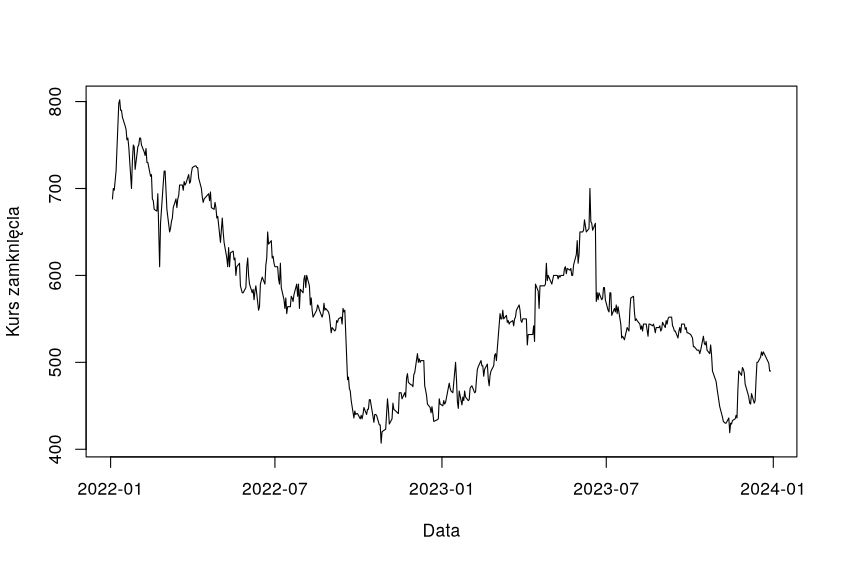
\includegraphics[width=1\textwidth]{./Kajtek/img/kursy_zamkniecia_plot.png}}

Zmianę log-zwrotów, wyliczonych według wzoru

$$ r_1 = \ln\frac{S_0}{S_1}, r_2 = \ln\frac{S_2}{S_1}, ..., r_n = \ln\frac{S_n}{S_{n-1}} $$

gdzie $s_0, s_1, ..., s_n$ są kursami zamknięcia z kolejnych dni, na osi czasu ilustruje wykres poniżej.

\centerline{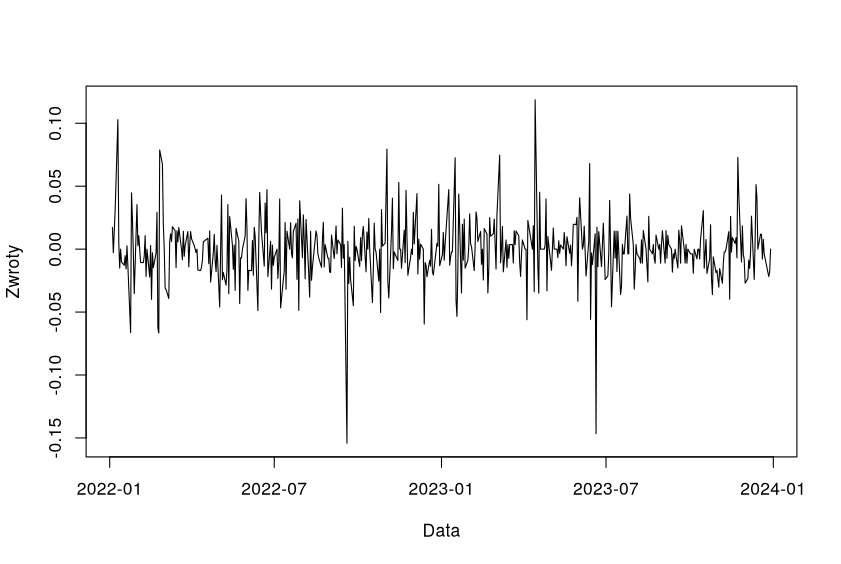
\includegraphics[width=1\textwidth]{./Kajtek/img/log_zwroty_plot.png}}


\subsubsection{Wartość oczekiwana:}
Zakładając, że log-zwroty $r_1, r_2, ..., r_n$ są niezależnymi realizacjami zmiennej losowej X, wyliczamy $\mu$ przy użyciu nieobciążonego estymatora wartości oczekiwanej:
$$ E(\overline{X}_n) = \frac{1}{n}\sum_{i=1}^{n}X_i = \mu $$
w wyniku czego otrzymujemy wynik 
$$\mu = -0.0006787669$$


\subsubsection{Wariancja i odchylenie standardowe:}
Korzystając ze wzoru na nieobciążony estymator wariancji
$$\sigma^{2}=\frac{1}{n-1}\sum_{i=1}^{n}(X_i - \overline{X}_n)^{2}$$
otrzymujemy $\sigma^{2}=0.0006189792$ oraz $\sigma=0.02487929$.
\subsubsection{Kwantyle:}
Z wykorzystaniem klasycznego estymatora kwantyli wyestymowano kwantyle rzędu $\alpha = 5\%, 50\% i 95\%$. Wyniki przedstawione zostaly w tabeli poniżej:
\begin{center}
\begin{tabular}{|c|c|c|c|c|c|}
    \hline
    $\overline{x}_n$ & $s_n^{2}$ & $s_n$ & $q(5\%)$ & $q(50\%)$ & $q(95\%)$ \\ \hline
    -0.0006787669 & 0.0006189792 & 0.02487929 & -0.03620640 & 0 & 0.04055989 \\ \hline
\end{tabular}
\end{center}


\subsubsection{Histogram log-zwrotów:}
Na histogramie dziennych log-zwrotów cen akcji na czerwono i niebiesko oznaczono odpowiednio wartość wyestymowanej średniej oraz wartości kwantyli przedstawionych wcześniej.

\centerline{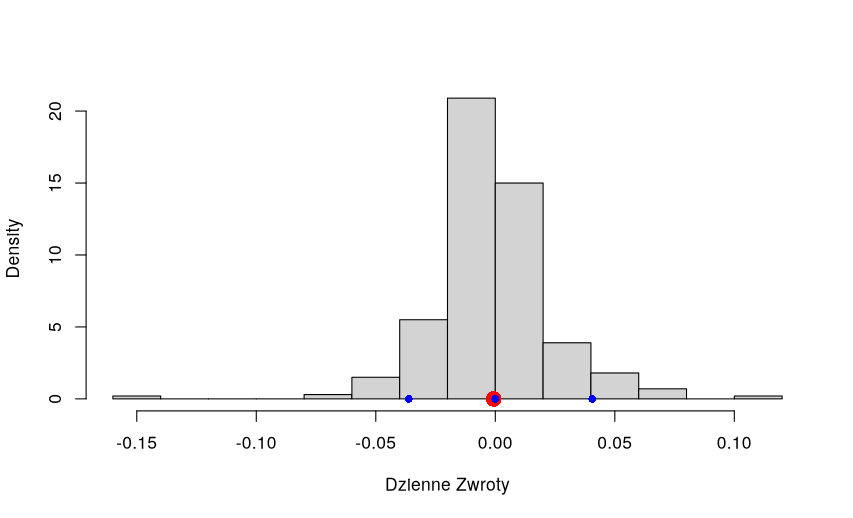
\includegraphics[width=1\textwidth]{./Kajtek/img/histogram_zwrotow.png}}


\newpage
\subsubsection{Dystrybuanta:}
Z wykorzystaniem dystrybuanty empirycznej jako nieobciążonego estymatora 

$$\hat{F}_n(x) = \frac{1}{n} \sum_{i=1}^{n} 1_\{x_i \leq x\} = \left(\frac{\text{liczba  elementów  w  próbie} \leq x}{n}\right)$$
estymujemy dystrybuantę F zaprezentowaną na wykresie poniżej

\centerline{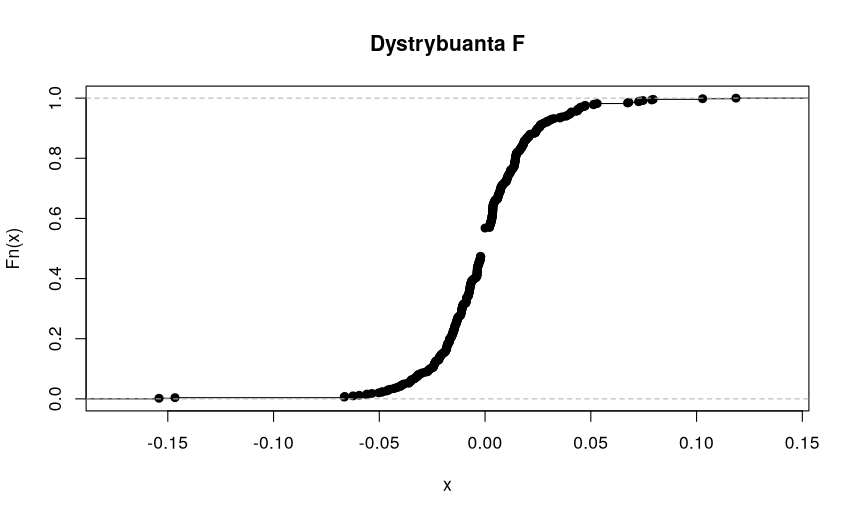
\includegraphics[width=1\textwidth]{./Kajtek/img/dystrybuanta.png}}

\subsubsection{Analiza dobroci dopasowania rozkładu normalnego i t-Studenta:}
Korzystając z \textbf{estymatora największej wiarygodności (MLE)} parametru estymujemy parametry rozkładu normalnego i t-Studenta.

% zapisac tu wzory
\begin{center}
\begin{tabular}{|c|c|c|}
    \hline
    $m$ & $s$ & $df$ \\ \hline
    -0.0006787669 & 0.0248544 & 314.3698 \\ \hline
\end{tabular}
\end{center}

\newpage
\subsubsection{Wykresy diagnostyczne}
Poniższe wykresy prezentują kolejno porównania: histogram-gęstość wybranych rozkładów, kwantyl-kwantyl, dystrybuanta empiryczna-dystrybuanta teoretyczna wybranych rozkładów oraz prawdopodobieństwo teoretyczne wybranych rozkładów-prawdopodobieństwo empiryczne.

\centerline{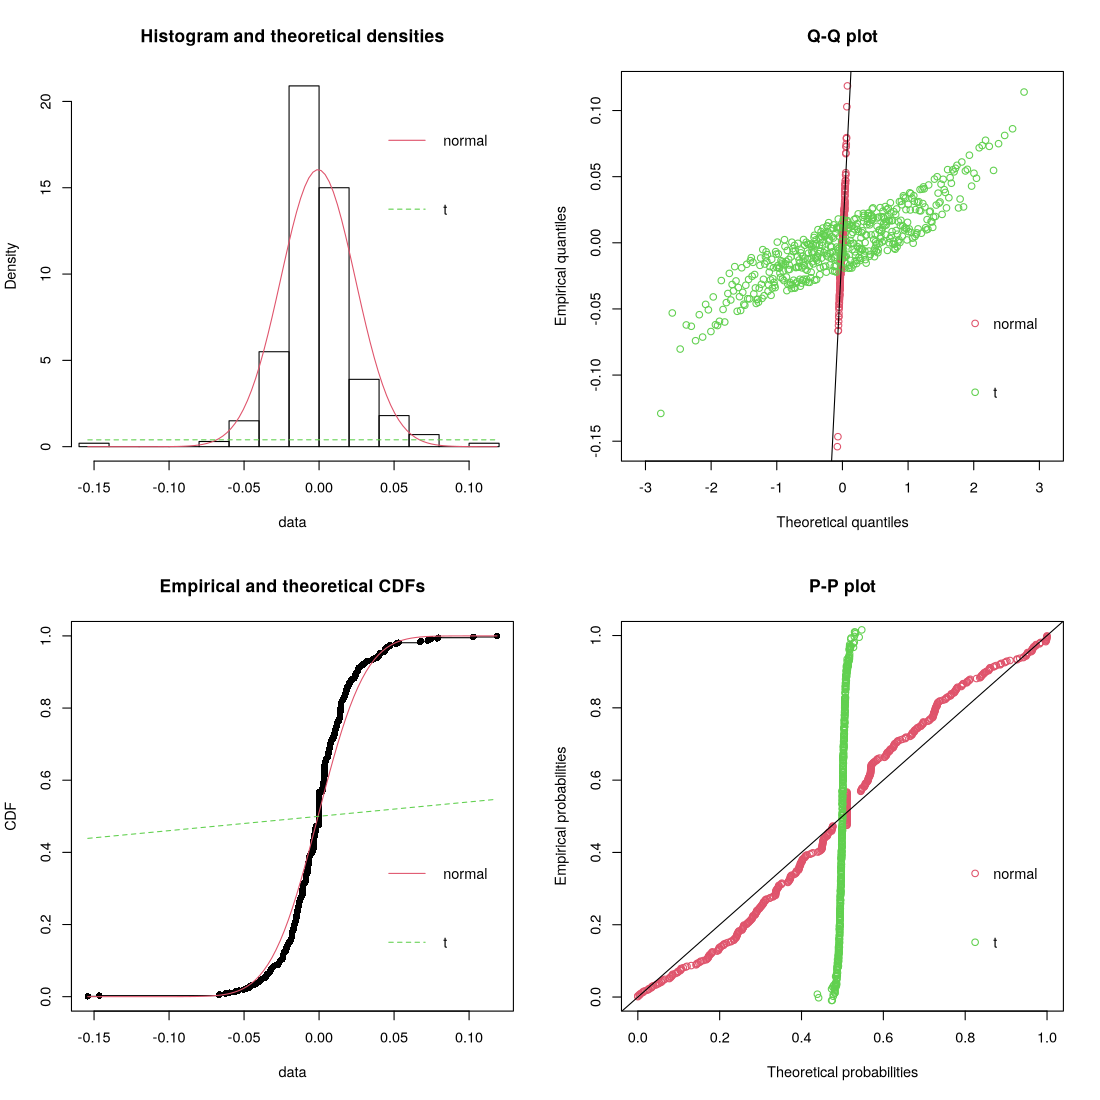
\includegraphics[width=1\textwidth]{./Kajtek/img/diagnostical-plots.png}}

Na ich podstawie można stwierdzić, że rozkład normalny lepiej dopasowuje się do danych.


\newpage
\subsubsection{Weryfikacja wyboru z wykorzystainem statystyk oraz kryteriów informacyjnych:}
Poniższe tabele prezentują wyniki testów statystycznych oraz kryteriów informacyjnych dla rozkładów normalnego i t-Studenta.

\begin{center}
\begin{tabular}{|c|c|c|}
    \hline
    Statystyki & Rozkład normalny & Rozkład t-Studenta  \\ \hline
    Kolmogorov-Smirnov & 0.08251589 & 0.469477 \\ \hline
    Cramer-von Mises & 1.18780300 & 39.177553 \\ \hline
    Anderson-Darling & 6.95700925 & 183.184800 \\ \hline
\end{tabular}
\end{center}

\begin{center}
\begin{tabular}{|c|c|c|}
    \hline
    Kryteria & Rozkład normalny & Rozkład t-Studenta  \\ \hline
    AIC & -2271.782 & 922.0439 \\ \hline
    BIC & -2263.353 & 926.2585 \\ \hline
\end{tabular}
\end{center}

Powyższe wyniki potwierdzają, że rozkład normalny lepiej dopasowuje się do danych.


\subsubsection{Test hipotezy równości rozkładów metodą Monte Carlo:}
Testujemy hipotezę zerową o równości dystrybuant
$$H_0: F = F_0$$
przeciwko hipotezie alternatywnej (kontrhipotezie)
$$H_1: F \neq F_0$$
gdzie $F_0$ jest dystrybuantą rozkładu normalnego wybranego w poprzedniej podsekcji, a F dystrybuantą nieznaną.
\newline Do przetestowania hipotezy zerowej o równości dystrybuant wykorzystamy metodę Monte Carlo przy użyciu statystyki Kołmogorowa-Smirnowa. 
\newline W tym celu generujemy $N=10000$ prób z rozkładu normalnego o parametrach 
$$m = -0.0006787669 \text{ oraz } s = 0.0248544$$ 
wyestymowanych wcześniej oraz obliczamy wartość statystyki Kołmogorowa-Smirnowa dla każdej z nich. 
\newline Następnie obliczamy prawdopodobieństwo 
$$p = P(D_n > d_n)$$ 
gdzie $D_n$ to wartość statystyki dla wygenerowanych prób a $d_n$ to jej wartość dla log-zwrotów spółki. 
\newline Ustalamy poziom istotności $\alpha = 0.05$ i sprawdzamy czy $p < \alpha$. W naszym przypadku 
$$p = 0.0025 < \alpha = 0.05$$ 
co pozwala nam odrzucić hipotezę zerową na rzecz hipotezy alternatywnej.

\subsection{Digitree}

\subsubsection{Wstęp}
Digitree to polska spółka technologiczna specjalizująca się w kompleksowych rozwiązaniach z zakresu digital marketingu i wsparcia sprzedaży online.


\subsubsection{Analiza log-zwrotów spółki DIGITREE}

\subsubsection{Spółka DIGITREE:}
Poniżej przedstawiam wykres kursów zamknięcia wybranej spółki

\centerline{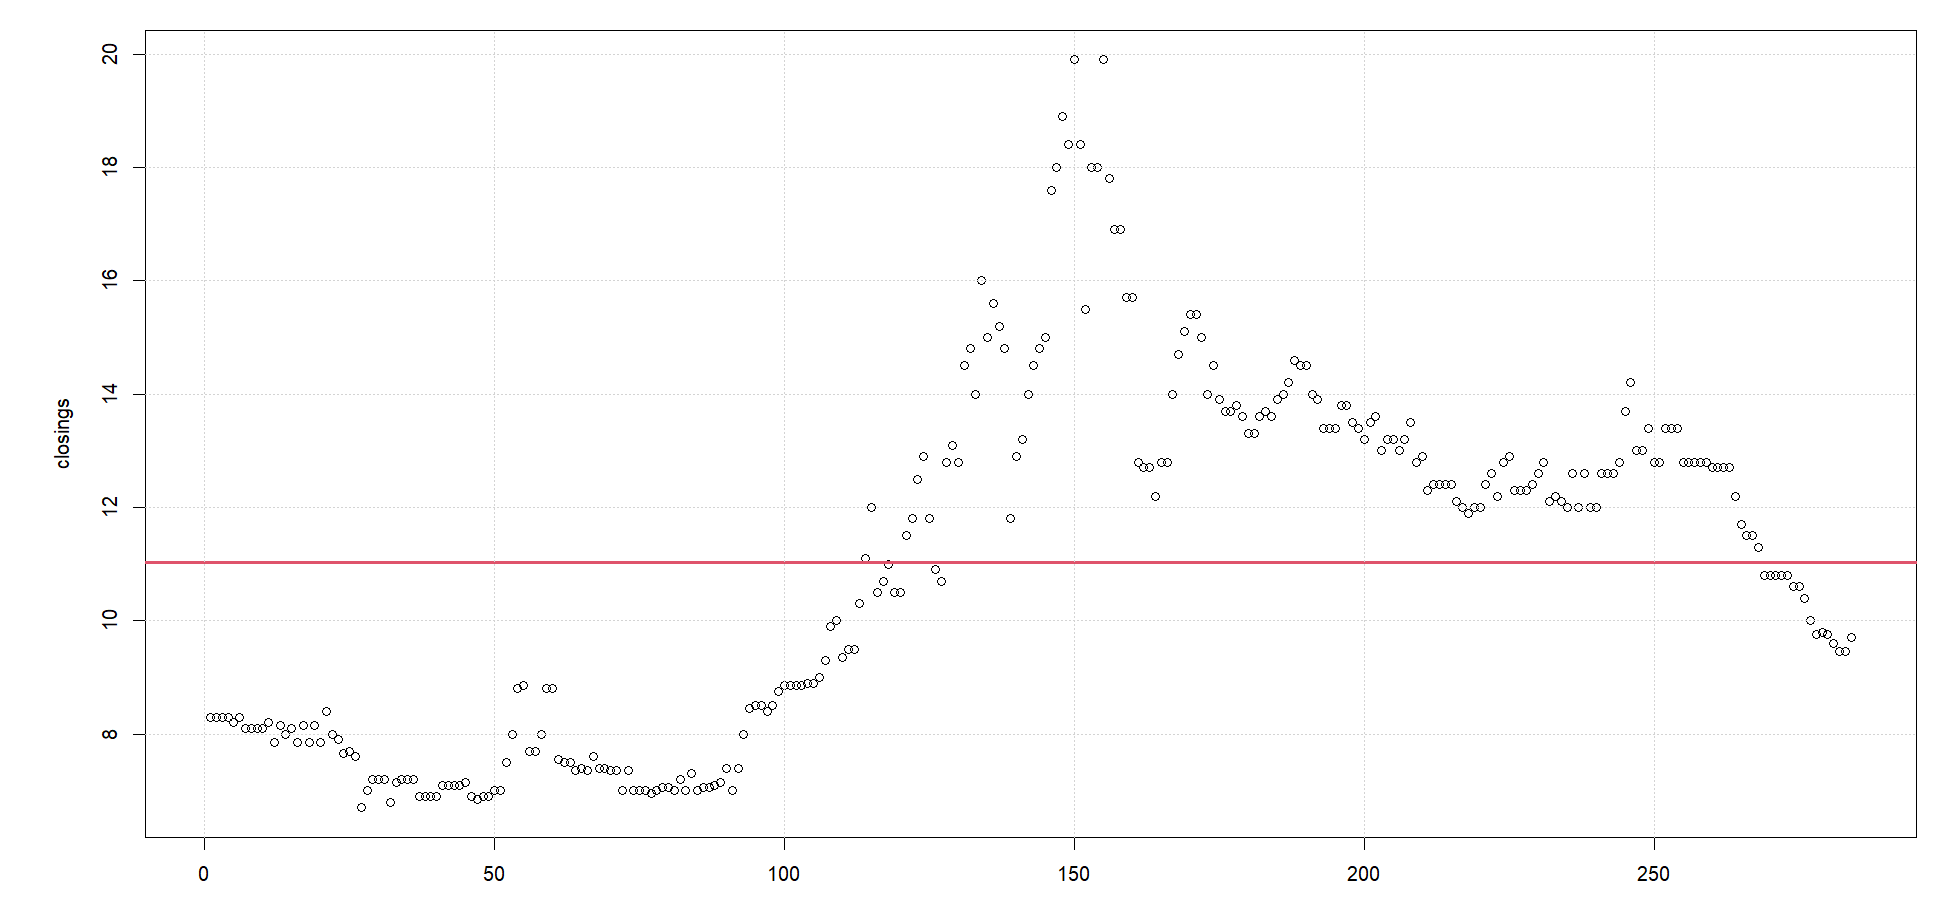
\includegraphics[width=14cm]{./Janek/zamkniecie.png}}

Poniżej przedstawiam wykres log-zwrotów wybranej spółki

\centerline{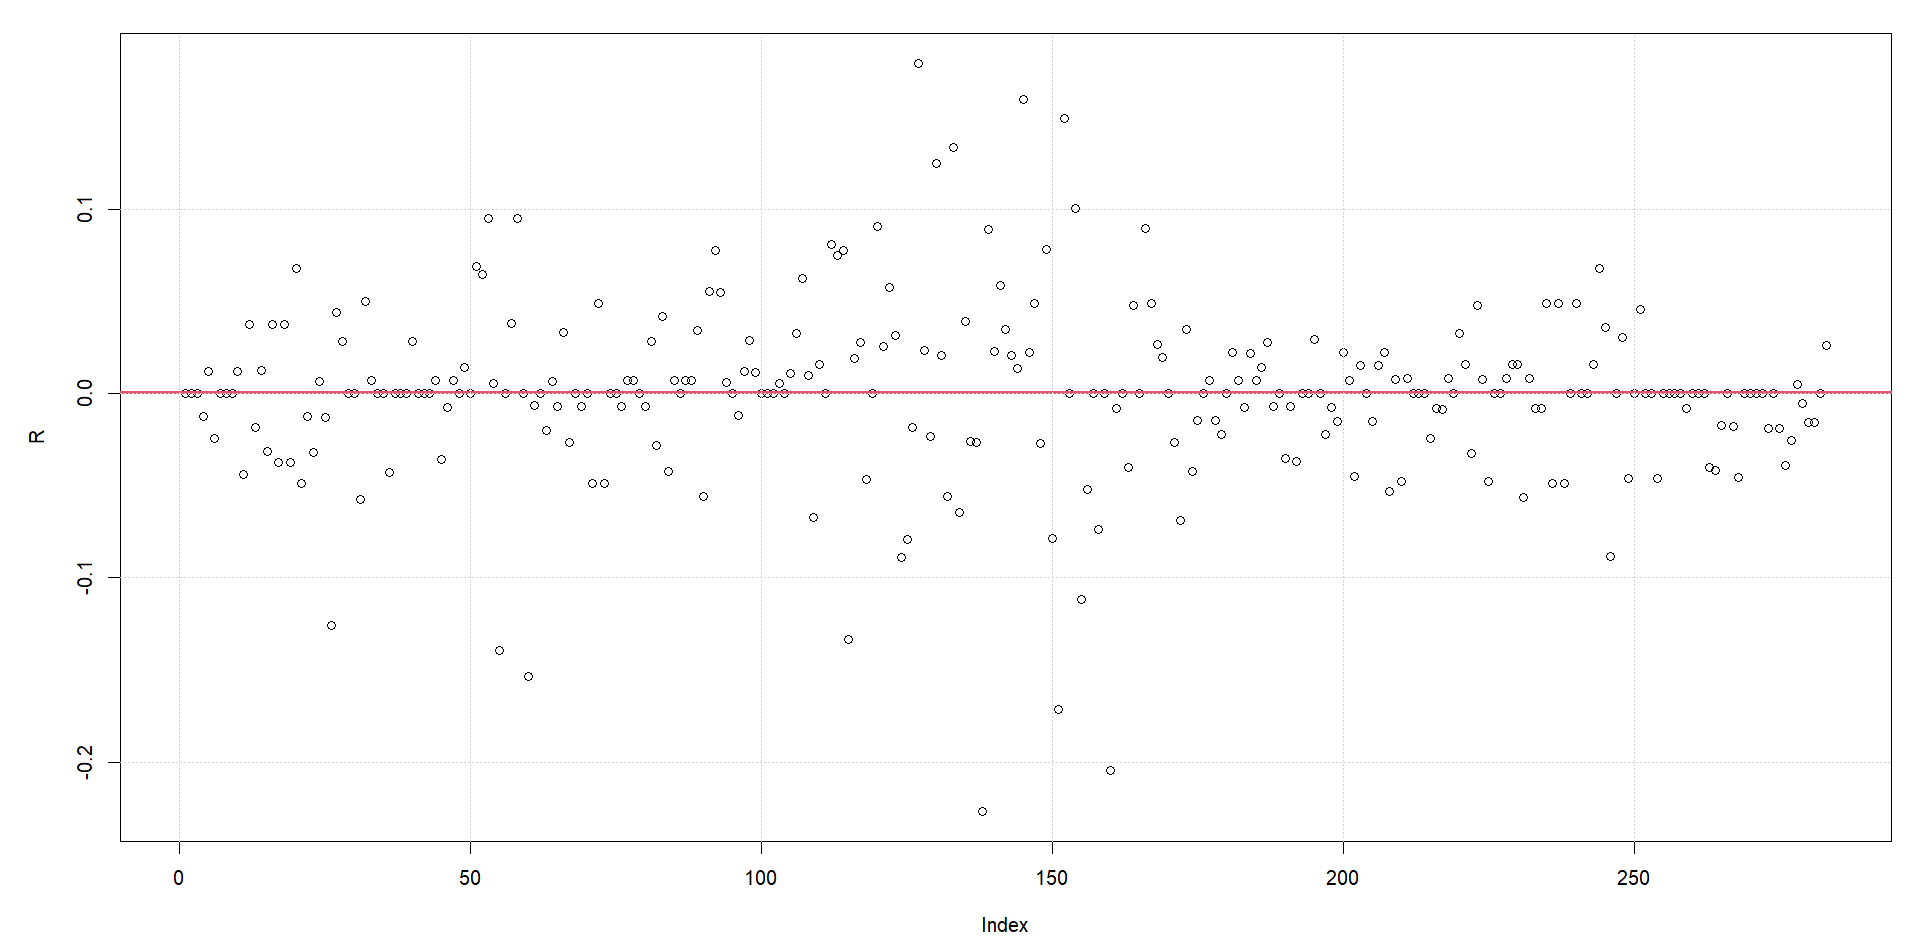
\includegraphics[width=14cm]{./Janek/logzwroty.png}}

wyliczonych według wzoru:

$$ r_1 = \ln\frac{S_0}{S_1}, r_2 = \ln\frac{S_2}{S_1}, ..., r_n = \ln\frac{S_n}{S_{n-1}} $$

gdzie $s_0, s_1, ..., s_n$ są kursami zamknięcia z kolejnych dni.

\subsubsection{Podstawowa analiza statystyczna log-zwrotów:}

Wartości log-zwrotów zostały obliczone jako różnice logarytmiczne dziennych kursów zamknięcia. Poniżej przedstawiono podstawowe statystyki log-zwrotów:

Zakładając, że log-zwroty $r_1, r_2, ..., r_n$ są niezależnymi realizacjami zmiennej losowej X, wyliczamy $\mu$ przy użyciu nieobciążonego estymatora wartości oczekiwanej:
$$ E(\overline{X}_n) = \frac{1}{n}\sum_{i=1}^{n}X_i = \mu $$
w wyniku czego otrzymujemy wynik 
$$\mu = 0.0005507787$$

Korzystając ze wzoru na nieobciążony estymator wariancji
$$\sigma^{2}=\frac{1}{n-1}\sum_{i=1}^{n}(X_i - \overline{X}_n)^{2}$$
otrzymujemy $\sigma^{2}=0.0022445$ oraz $\sigma=0.04737616$.

\begin{table}[h!]
\centering
\caption{Estymacja parametrów log-zwrotów}
\begin{tabular}{|c|c|c|c|c|c|}
\hline
$\overline{x}_n$ & $s^2_n$ & $s_n$ & $q(5\%)$ & $q(50\%)$ & $q(95\%)$ \\ \hline
0.0005507787 & 0.0022445 & 0.04737616 & -0.06694173 & 0.00000000 & 0.07764551 \\ \hline
\end{tabular}
\end{table}

Kwantyle 5\%, 50\%, i 95\% przedstawiają odpowiednio wartości, poniżej których znajduje się odpowiednio 5\%, 50\%, i 95\% log-zwrotów. Na przykład, wartość kwantyla 5\% oznacza, że 5\% log-zwrotów jest mniejszych od -0.0669.

\subsubsection{Histogram log-zwrotów z zaznaczoną średnią i kwantylami:}

Poniżej zamieszczono histogram log-zwrotów z zaznaczonymi wartościami średniej oraz kwantyli 5\%, 50\% i 95\%.

\centerline{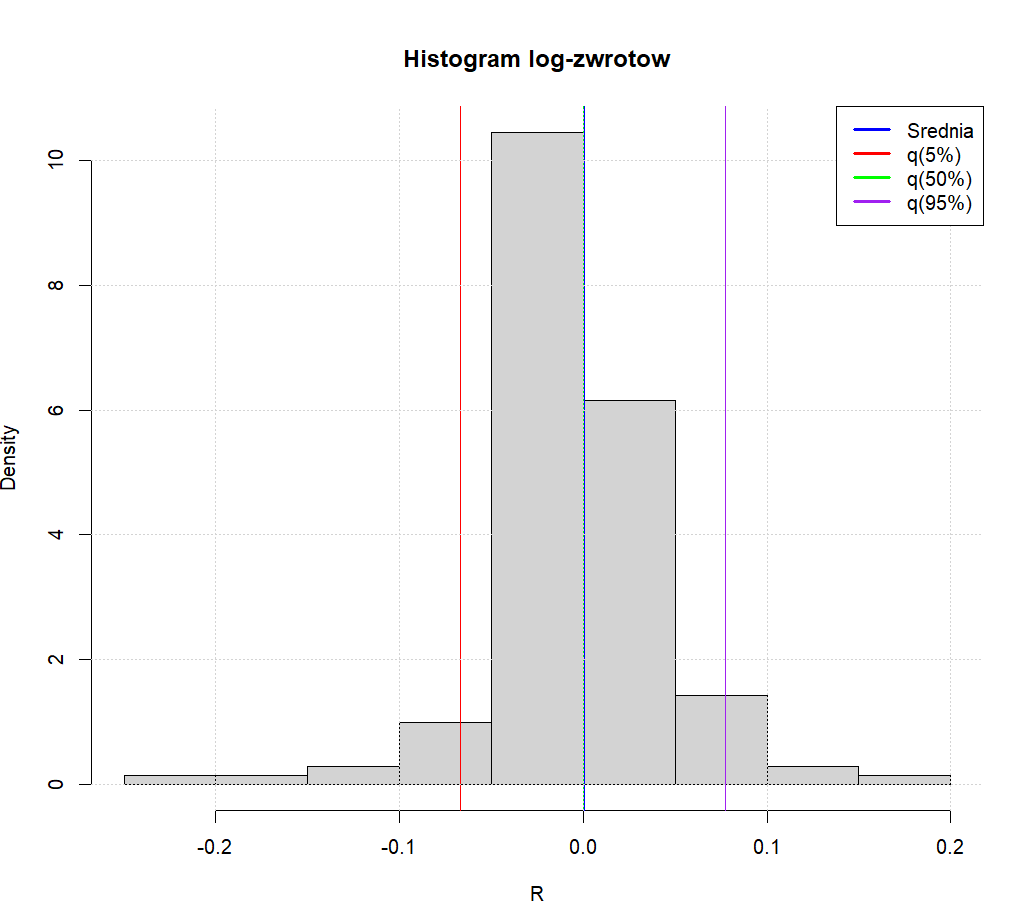
\includegraphics[width=14cm]{./Janek/histogram logzwrotow.png}}

\subsubsection{Dystrybuanta empiryczna log-zwrotów:}

Estymacja dystrybuanty empirycznej dla log-zwrotów została przeprowadzona przy użyciu wzoru empirycznej dystrybuanty $F_n(x)$:

$$\hat{F}_n(x) = \frac{1}{n} \sum_{i=1}^{n} 1_\{x_i \leq x\} = \left(\frac{\text{liczba  elementów  w  próbie} \leq x}{n}\right)$$
wykres dystrybuanty empirycznej log-zwrotów znajduje się poniżej.

\centerline{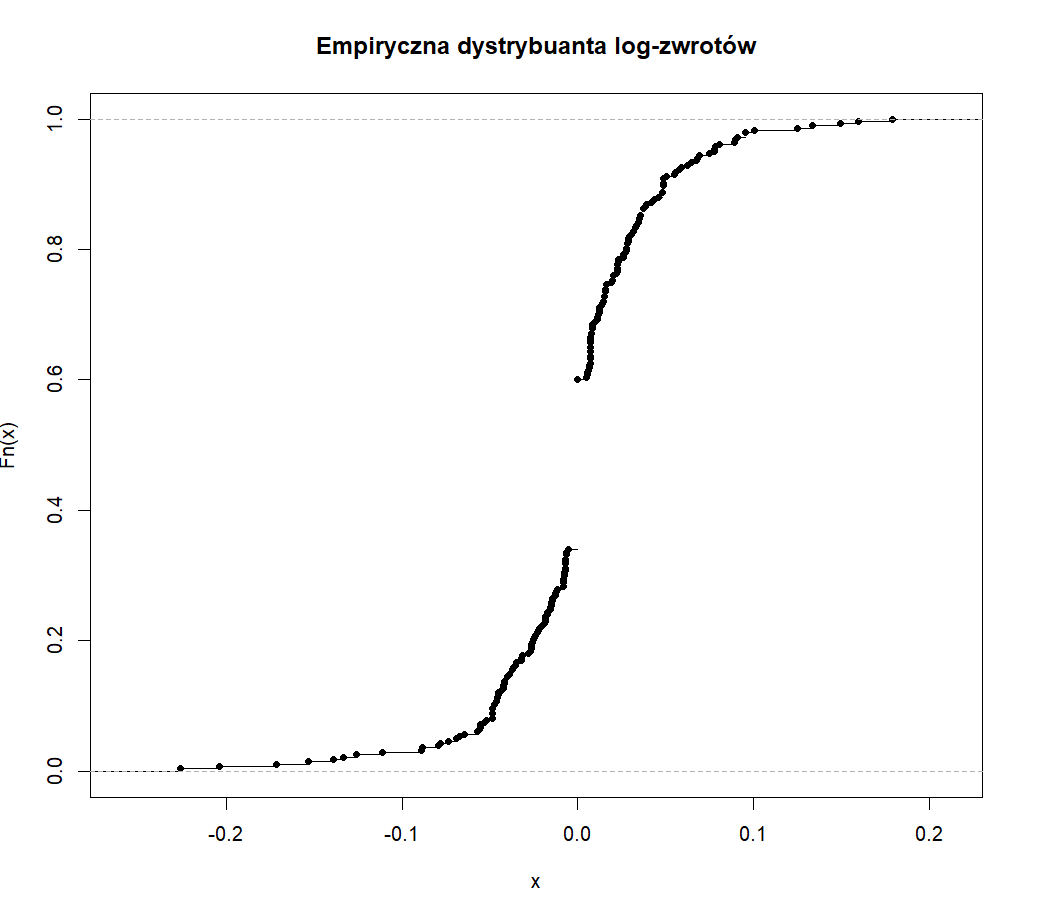
\includegraphics[width=14cm]{./Janek/empiryczna dystrybuanta.png}} 

\subsubsection{Analiza dobroci dopasowania rozkładów}

\subsubsection{Estymacja parametrów rozkładu normalnego i t-Studenta:}

Parametry rozkładu normalnego i t-Studenta zostały wyestymowane przy użyciu estymatora największej wiarygodności (MLE):
\begin{itemize}
    \item Rozkład normalny: średnia = 0.0005507787, odchylenie standardowe = 0.0472923802
    \item Rozkład t-Studenta: liczba stopni swobody = 307.2041
\end{itemize}

\subsubsection{Wykresy diagnostyczne:}

Poniżej przedstawiono wykresy diagnostyczne dla dopasowania rozkładów normalnego i t-Studenta do danych log-zwrotów, umożliwiające ocenę jakości dopasowania.

\centerline{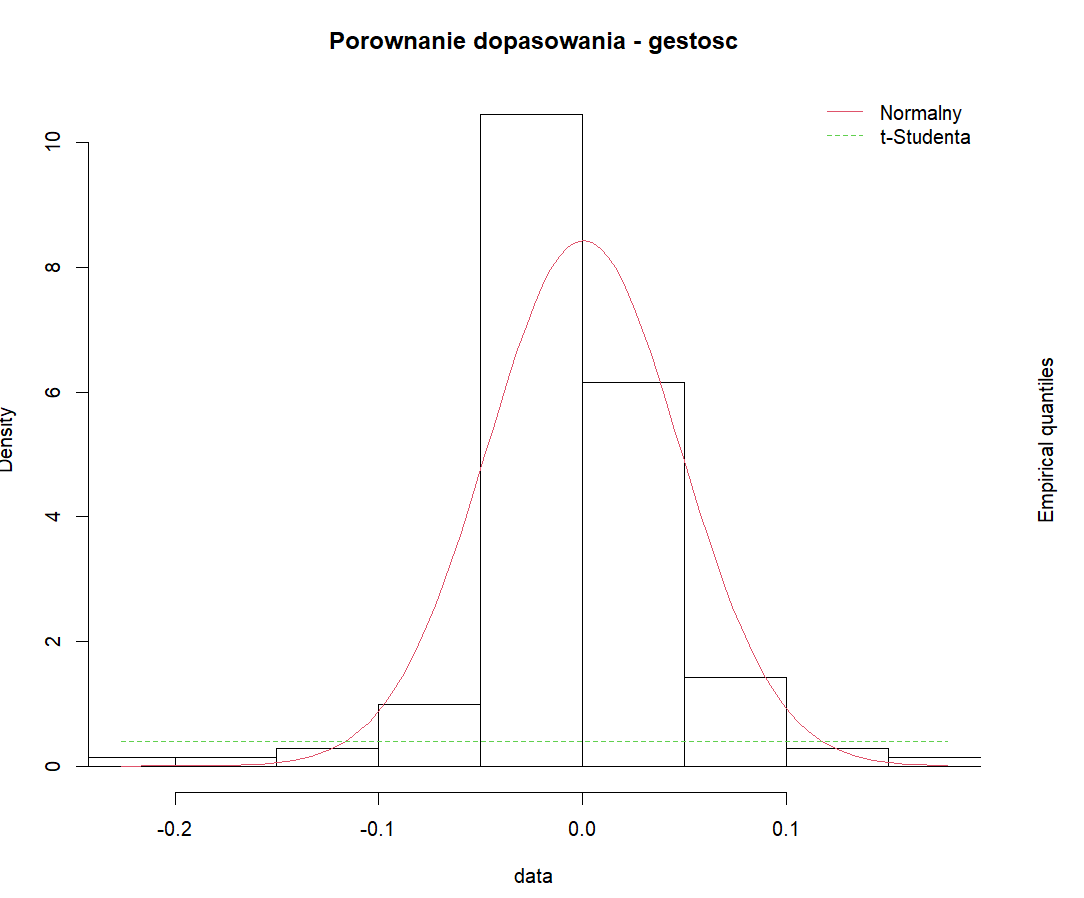
\includegraphics[width=14cm]{./Janek/dopasowanie gestosc.png}}
\centerline{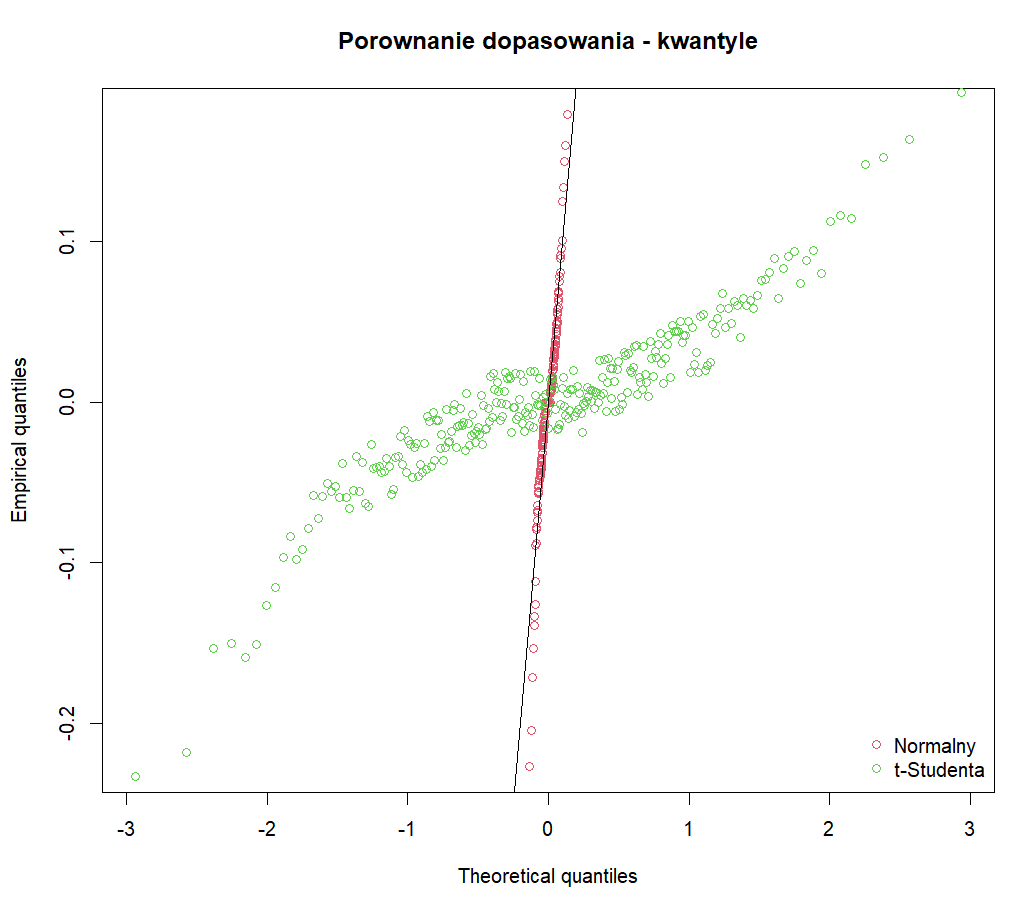
\includegraphics[width=14cm]{./Janek/dopasowanie kwantyle.png}} 
\centerline{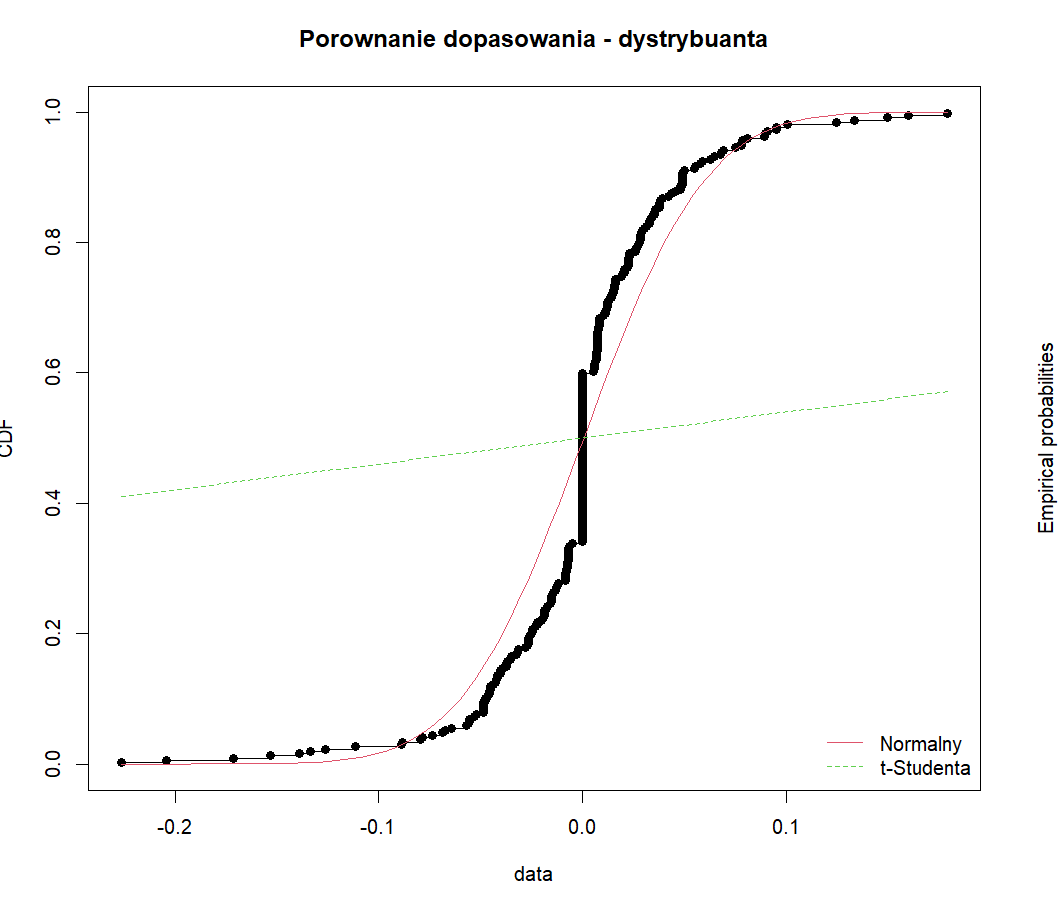
\includegraphics[width=14cm]{./Janek/dopasowanie dystrybuanta.png}}
\centerline{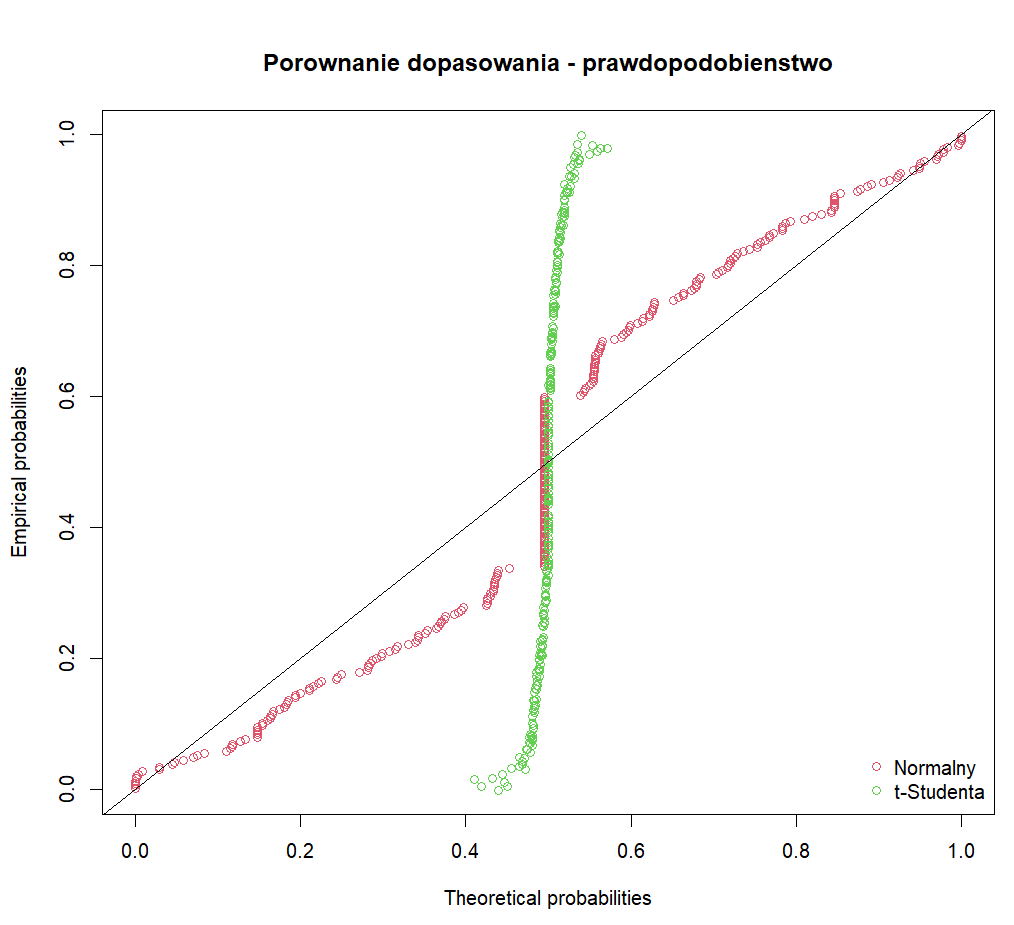
\includegraphics[width=14cm]{./Janek/dopasowanie pradopodobienstwo.png}} 

\subsubsection{Ocena dopasowania rozkładów}

Na podstawie wykresów diagnostycznych oraz statystyk dopasowania:
\begin{itemize}
    \item Statystyki dla rozkładu normalnego: KS = 0.1561, CM = 1.8659, AD = 9.3673, AIC = -919.9766, BIC = -912.6857
    \item Statystyki dla rozkładu t-Studenta: KS = 0.4424, CM = 21.0334, AD = 99.0999, AIC = 523.2149, BIC = 526.8603
\end{itemize}

Wyniki sugerują, że rozkład normalny lepiej dopasowuje się do danych log-zwrotów niż rozkład t-Studenta. Wybór rozkładu normalnego uzasadniają niższe wartości AIC i BIC oraz lepsze dopasowanie na wykresach diagnostycznych.

\subsubsection{Test hipotezy o równości rozkładów:}

Przeprowadzono test hipotezy o równości rozkładów dla wybranego rozkładu normalnego, wykorzystując statystykę Kolmogorova-Smirnova (KS) z wykorzystaniem N = 10000 prób z rozkładu normalnego. Wyniki testu przedstawiono poniżej:

\begin{itemize}
    \item \textbf{Statystyka testowa \( D \):} Obliczona wartość wynosi \( D = 0.1561313 \). Statystyka \( D \) mierzy maksymalną różnicę pomiędzy dystrybuantą empiryczną danych a teoretyczną dystrybuantą rozkładu normalnego. Wysoka wartość \( D \) wskazuje na większą różnicę, co może sugerować, że dane nie pochodzą z badanego rozkładu.
    \item \textbf{P-wartość (\( p \)):} Obliczona p-wartość wynosi \( p = 0 \). Oznacza to, że przy założeniu prawdziwości hipotezy zerowej, prawdopodobieństwo uzyskania tak dużej lub większej różnicy \( D \) wynosi praktycznie zero. W rezultacie, hipoteza zerowa o zgodności rozkładu danych z rozkładem normalnym zostaje odrzucona na dowolnym poziomie istotności.
\end{itemize}

\textbf{Interpretacja:}
\begin{itemize}
    \item Obliczona wartość statystyki \( D \) sugeruje, że istnieją istotne różnice pomiędzy rozkładem danych a teoretycznym rozkładem normalnym. 
    \item Niska p-wartość (\( p = 0 \)) wskazuje, że te różnice są statystycznie istotne. Oznacza to, że dane najprawdopodobniej nie pochodzą z badanego rozkładu normalnego.
\end{itemize}

\subsection{Wawel}

\subsubsection{Wprowadzenie}
Wawel SA (WWL) jest polskim producentem słodyczy, znanym z produkcji czekolad, cukierków, wafli oraz innych wyrobów cukierniczych. Firma cieszy się długą tradycją na rynku i dostarcza wysokiej jakości produkty konsumentom zarówno w Polsce, jak i za granicą.

Przeprowadzona analiza stanowi pierwszą część projektu zaliczeniowego, w której skupimy się na analizie log-zwrotów akcji spółki Wawel SA.

\subsubsection{Wykresy kursów zamknięcia oraz log-zwrotów}

\begin{figure}[H]
    \centering
    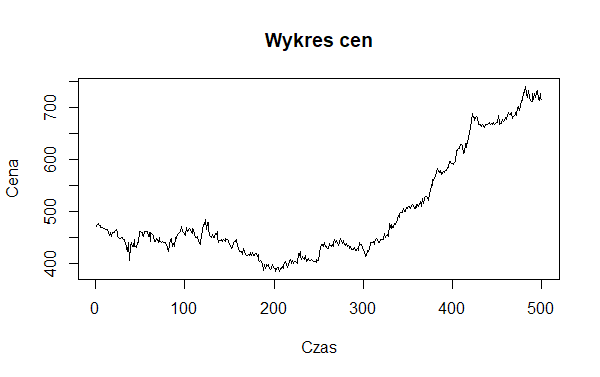
\includegraphics[width=0.8\textwidth]{./Wojtek/wykres-cen.png}
    \caption{Wykres cen akcji spółki Wawel SA (WWL)}
    \label{fig:wykres_cen}
\end{figure}

\begin{figure}[H]
    \centering
    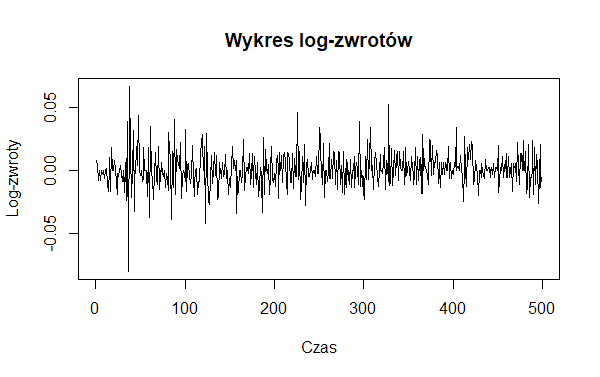
\includegraphics[width=0.8\textwidth]{./Wojtek/wykres-log-zwrotow.png}
    \caption{Wykres log-zwrotów akcji spółki Wawel SA (WWL)}
    \label{fig:wykres_log_zwrotow}
\end{figure}

Wykresy powyżej ilustrują zmiany kursów zamknięcia oraz log-zwrotów akcji spółki Wawel SA w czasie. Widać na nich zmienność cen akcji oraz ich wpływ na log-zwroty.

\subsubsection{Analiza log-zwrotów}
Zakładamy, że log-zwroty $r_1, r_2, \ldots, r_n$ są niezależnymi realizacjami zmiennej losowej $X$ o dystrybuancie $F$, wartości oczekiwanej $\mu$ i wariancji $\sigma^2$. 

Odpowiednie estymatory użyte w analizie to:
\begin{equation}
    \hat{\mu} = \frac{1}{n} \sum_{i=1}^{n} r_i
\end{equation}
\begin{equation}
    \hat{\sigma}^2 = \frac{1}{n-1} \sum_{i=1}^{n} (r_i - \hat{\mu})^2
\end{equation}
\begin{equation}
    \hat{\sigma} = \sqrt{\hat{\sigma}^2}
\end{equation}

Korzystając z klasycznego estymatora kwantyli, wyestymowano kwantyle rzędu $\alpha = 5\%, 50\%, 95\%$. Wyniki zostały przedstawione w tabeli poniżej:

\begin{table}[H]
    \centering
    \begin{tabular}{|l|r|}
        \hline
        \textbf{Estymator} & \textbf{Wartość} \\
        \hline
        Liczność próby ($n$) & 499 \\
        Wartość oczekiwana ($\hat{\mu}$) & 0,000837 \\
        Wariancja ($\hat{\sigma}^2$) & 0,000202 \\
        Odchylenie standardowe ($\hat{\sigma}$) & 0,014220 \\
        Kwantyl 5\% ($q_{5\%}$) & -0,020416 \\
        Kwantyl 50\% ($q_{50\%}$) & 0,000000 \\
        Kwantyl 95\% ($q_{95\%}$) & 0,023786 \\
        \hline
    \end{tabular}
    \caption{Podstawowe statystyki log-zwrotów akcji spółki Wawel SA (WWL)}
    \label{tab:wyniki}
\end{table}

\begin{figure}[H]
    \centering
    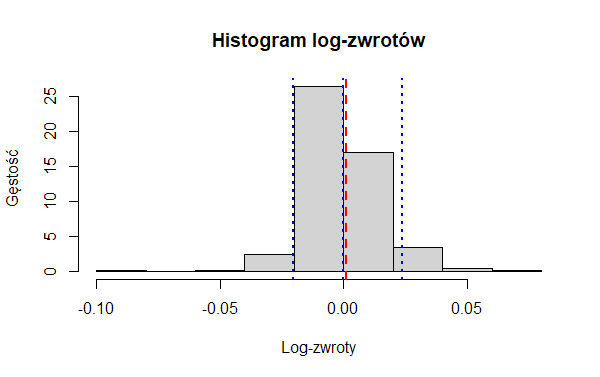
\includegraphics[width=0.8\textwidth]{./Wojtek/histogram-log-zwrotow.png}
    \caption{Histogram log-zwrotów z zaznaczoną średnią i kwantylami}
    \label{fig:histogram_log_zwrotow}
\end{figure}

\subsubsection{Interpretacja kwantyli}
Każdy z kwantyli ma swoją specyficzną interpretację w kontekście log-zwrotów akcji:
\begin{itemize}
    \item \textbf{Kwantyl 5\%}: Wartość log-zwrotu, poniżej której znajduje się 5\% najmniejszych obserwacji. Oznacza to, że istnieje 5\% szans, że log-zwrot będzie niższy niż -0,020416.
    \item \textbf{Kwantyl 50\% (mediana)}: Wartość środkowa log-zwrotów. Oznacza to, że połowa log-zwrotów jest większa, a połowa mniejsza niż 0,000000.
    \item \textbf{Kwantyl 95\%}: Wartość log-zwrotu, poniżej której znajduje się 95\% obserwacji. Oznacza to, że tylko 5\% log-zwrotów jest wyższych niż 0,023786.
\end{itemize}

\subsubsection{Estymacja dystrybuanty}
W celu estymacji dystrybuanty $F$ wykorzystano empiryczny estymator dystrybuanty, którego wzór jest następujący:
\begin{equation}
    \hat{F}(x) = \frac{1}{n} \sum_{i=1}^{n} I(r_i \leq x),
\end{equation}
 gdzie $I(r_i \leq x)$ jest funkcją indykatora, a $n$ oznacza liczbę obserwacji.

Dystrybuanta empiryczna została przedstawiona na wykresie poniżej:

\begin{figure}[H]
    \centering
    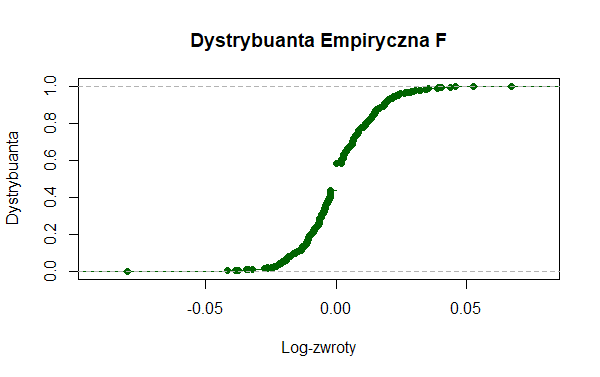
\includegraphics[width=0.8\textwidth]{./Wojtek/dystrybuanta-empiryczna.png}
    \caption{Dystrybuanta empiryczna $\hat{F}(x)$ dla log-zwrotów}
    \label{fig:dystrybuanta_empiryczna}
\end{figure}

\subsubsection{Analiza dobroci dopasowania rozkładu normalnego i t-Studenta}

\subsubsection{Estymacja parametrów:}

Wykorzystując estymator największej wiarygodności (MLE) oraz bibliotekę \texttt{fitdistrplus} w R, wyestymowano parametry rozkładu normalnego i t-Studenta dla danych log-zwrotów.

\subsubsection{Rozkład normalny}

\begin{table}[H]
    \centering
    \begin{tabular}{|l|r|r|}
        \hline
        & \textbf{Estymata} & \textbf{Błąd standardowy} \\
        \hline
        Średnia ($\hat{\mu}$) & 0,000837 & 0,000636 \\
        Odchylenie standardowe ($\hat{\sigma}$) & 0,014205 & 0,000440 \\
        \hline
    \end{tabular}
    \caption{Estymowane parametry rozkładu normalnego}
    \label{tab:fit_norm}
\end{table}

\subsubsection{Rozkład t-Studenta}

\begin{table}[H]
    \centering
    \begin{tabular}{|l|r|r|}
        \hline
        & \textbf{Estymata} & \textbf{Błąd standardowy} \\
        \hline
        Liczba stopni swobody ($\hat{\nu}$) & 4,9764 & 1,1504 \\
        Średnia ($\hat{\mu}$) & 0,000344 & 0,000578 \\
        Skala ($\hat{\sigma}$) & 0,011042 & 0,000611 \\
        \hline
    \end{tabular}
    \caption{Estymowane parametry rozkładu t-Studenta}
    \label{tab:fit_t}
\end{table}

\subsubsection{Wykresy diagnostyczne}

\subsubsection{Histogram z nałożonymi gęstościami}

\begin{figure}[H]
    \centering
    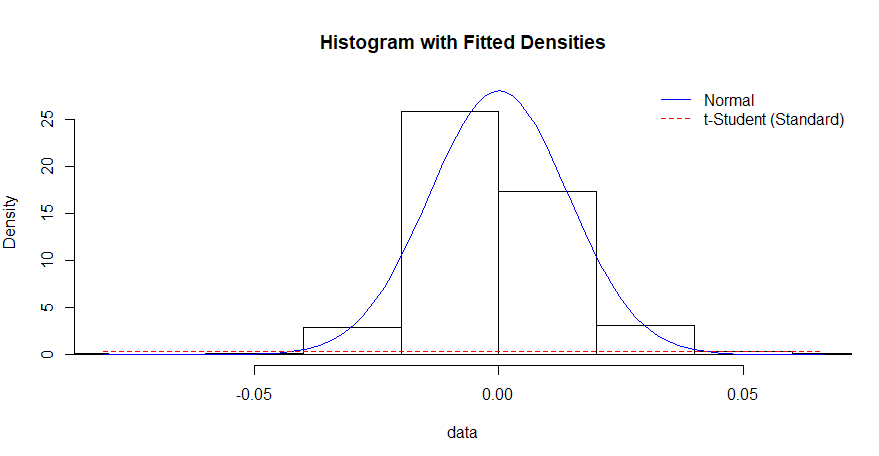
\includegraphics[width=0.8\textwidth]{./Wojtek/histogram-z-gestosciami.png}
    \caption{Histogram log-zwrotów z nałożonymi funkcjami gęstości rozkładów normalnego i t-Studenta}
    \label{fig:histogram_gestosci}
\end{figure}

\textbf{Opis:} Wykres histogramu przedstawia empiryczny rozkład danych, na który nałożono dopasowane gęstości rozkładów normalnego (niebieska linia) i t-Studenta (czerwona linia przerywana).  
Analiza wykazuje, że:
\begin{itemize}
    \item Rozkład normalny (niebieski) lepiej odwzorowuje dane empiryczne, szczególnie w centralnym zakresie wartości.
    \item Rozkład t-Studenta (czerwony) jest znacząco niedopasowany.
\end{itemize}

\subsubsection{Wykres kwantyl-kwantyl (Q-Q plot)}

\begin{figure}[H]
    \centering
    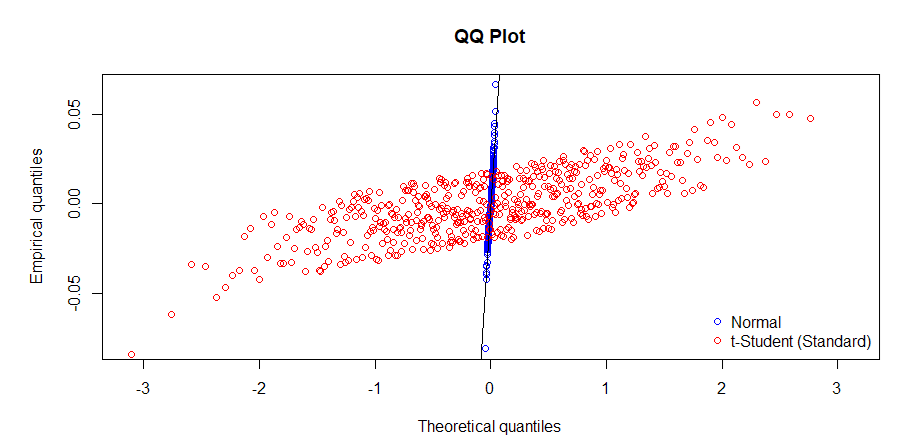
\includegraphics[width=0.8\textwidth]{./Wojtek/wykres-kwantyl-kwantyl.png}
    \caption{Wykres Q-Q dla rozkładów normalnego i t-Studenta}
    \label{fig:qq_plot}
\end{figure}

\textbf{Opis:} Wykres QQ porównuje kwantyle empiryczne danych z kwantylami teoretycznymi rozkładów normalnego i t-Studenta.  
Na wykresie zauważalne są następujące cechy:
\begin{itemize}
    \item Punkty dla rozkładu normalnego (niebieskie) układają się niemal idealnie wzdłuż linii prostej, co sugeruje wysoką zgodność z danymi empirycznymi.
    \item Rozkład t-Studenta (czerwony) znacznie odstaje od linii prostej, wskazując na niedopasowanie tego rozkładu do danych.
\end{itemize}

\subsubsection{Porównanie dystrybuant (CDF)}

\begin{figure}[H]
    \centering
    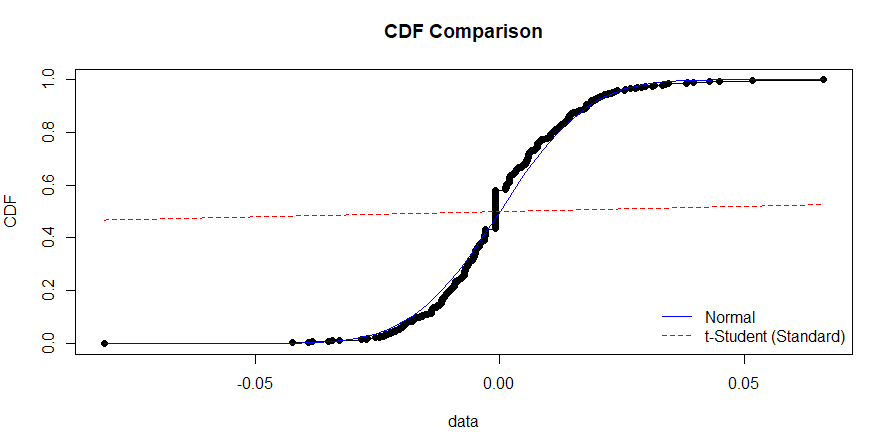
\includegraphics[width=0.8\textwidth]{./Wojtek/dystrybuanta-empiryczna-vs-teoretyczna.png}
    \caption{Porównanie dystrybuant empirycznej z teoretycznymi dla rozkładów normalnego i t-Studenta}
    \label{fig:dystrybuanta_vs_teoretyczna}
\end{figure}

\textbf{Opis:} Wykres porównuje empiryczną dystrybuantę danych z teoretycznymi dystrybuantami rozkładów normalnego i t-Studenta.  
Główne obserwacje:
\begin{itemize}
    \item Dystrybuanta rozkładu normalnego (niebieska linia) doskonale pokrywa się z empiryczną dystrybuantą danych.
    \item Dystrybuanta rozkładu t-Studenta (czerwona linia przerywana) wykazuje znaczne rozbieżności, co wskazuje na niedopasowanie.
\end{itemize}

\subsubsection{Wykres P-P (Probability-Probability plot)}

\begin{figure}[H]
    \centering
    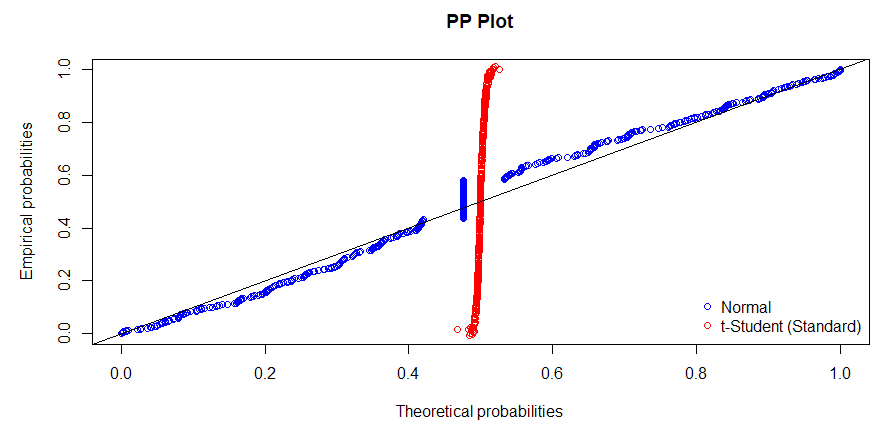
\includegraphics[width=0.8\textwidth]{./Wojtek/wykres-pp.png}
    \caption{Wykres P-P dla rozkładów normalnego i t-Studenta}
    \label{fig:pp_plot}
\end{figure}

\textbf{Opis:} Wykres PP ilustruje zgodność empirycznych prawdopodobieństw z teoretycznymi dla rozkładu normalnego. Natomiast dane rozkładu T-Studenta znacząco odbiegają od danych rzeczywistych.  
Z analizy wynika:
\begin{itemize}
    \item Punkty dla rozkładu normalnego (niebieskie) układają się niemal idealnie wzdłuż linii przekątnej, co potwierdza bardzo dobre dopasowanie do danych.
    \item Rozkład t-Studenta (czerwony) pokazuje znaczne odstępstwa od linii przekątnej, co sugeruje istotne niedopasowanie.
\end{itemize}

\subsubsection{Ocena dopasowania rozkładów}

Analiza jednoznacznie wskazuje, że dane empiryczne są znacznie lepiej modelowane przez rozkład \textbf{normalny} niż przez rozkład t-Studenta.  
\textbf{Wnioski:}
\begin{itemize}
    \item Rozkład normalny charakteryzuje się bliskim dopasowaniem zarówno w centralnej części, jak i w ogonach.
    \item Rozkład t-Studenta znacząco odbiega od danych, co czyni go nieodpowiednim w tym przypadku.
\end{itemize}

\newpage\subsubsection*{Interpretacja statystyk dopasowania rozkładów}

\subsubsection*{Statystyki dopasowania (\textit{Goodness-of-fit statistics})}

\begin{table}[h!]
\centering
\begin{tabular}{|l|c|c|}
\hline
\textbf{Statystyka}            & \textbf{Normalny} & \textbf{t-Studenta} \\ \hline
Kolmogorov-Smirnov             & 0.1047            & 0.4811             \\ \hline
Cramer-von Mises               & 0.6771            & 40.0829            \\ \hline
Anderson-Darling               & 3.5170            & 186.7583           \\ \hline
\end{tabular}
\caption{Porównanie statystyk dopasowania rozkładów}
\end{table}

\textbf{Interpretacja:}
\begin{itemize}
    \item Rozkład normalny uzyskał znacznie niższe wartości dla wszystkich trzech statystyk, co wskazuje na lepsze dopasowanie do danych w porównaniu z rozkładem t-Studenta.
    \item Szczególnie wartość statystyki Andersona-Darlinga dla rozkładu t-Studenta ($186.7583$) podkreśla jego niedopasowanie.
\end{itemize}

\subsubsection*{Kryteria dopasowania (\textit{Goodness-of-fit criteria})}

\begin{table}[h!]
\centering
\begin{tabular}{|l|c|c|}
\hline
\textbf{Kryterium}                     & \textbf{Normalny} & \textbf{t-Studenta} \\ \hline
Akaike's Information Criterion (AIC)  & -2825.534         & 919.8094            \\ \hline
Bayesian Information Criterion (BIC)  & -2817.109         & 924.0220            \\ \hline
\end{tabular}
\caption{Porównanie kryteriów dopasowania rozkładów}
\end{table}

\textbf{Interpretacja:}
\begin{itemize}
    \item Zarówno kryterium Akaike'go (AIC), jak i kryterium Bayesowskie (BIC) wskazują, że rozkład normalny jest znacznie lepiej dopasowany niż rozkład t-Studenta.
    \item Niższe wartości dla rozkładu normalnego ($-2825.534$ dla AIC oraz $-2817.109$ dla BIC) wskazują na przewagę tego modelu w uwzględnianiu dopasowania i prostoty modelu.
\end{itemize}

\subsubsection*{Podsumowanie}

Na podstawie przedstawionych statystyk i kryteriów dopasowania:
\begin{itemize}
    \item Rozkład \textbf{normalny} jest znacznie lepszy w modelowaniu danych niż rozkład t-Studenta.
    \item Rozkład t-Studenta charakteryzuje się dużymi odstępstwami w dopasowaniu, co czyni go nieodpowiednim w tym przypadku.
\end{itemize}



\newpage\subsubsection{Test hipotezy metodą Monte Carlo}

Dla wybranego rozkładu t-Studenta przeprowadzono test hipotezy o równości rozkładów, wykorzystując statystykę Kolmogorowa-Smirnowa (KS) oraz metodę Monte Carlo. Wyniki testu przedstawiono w tabeli 5.

\begin{table}[H]
    \centering
    \begin{tabular}{|p{7cm}|c|}
        \hline
        \textbf{Wynik} & \textbf{Wartość} \\
        \hline
        Zaobserwowana statystyka KS & 0,0893735 \\
        P-wartość z symulacji Monte Carlo & 0 \\
        \hline
    \end{tabular}
    \caption{Wyniki testu hipotezy metodą Monte Carlo}
    \label{tab:test_results}
\end{table}


\textbf{Interpretacja:} P-wartość równa 0 wskazuje na silne podstawy do odrzucenia hipotezy zerowej, że dane pochodzą z rozkładu t-Studenta z wyestymowanymi parametrami. Oznacza to, że mimo lepszego dopasowania w porównaniu z rozkładem normalnym, rozkład t-Studenta nie jest w stanie w pełni opisać danych log-zwrotów.

\subsubsection*{Histogram logarytmicznych zwrotów}

\textbf{Opis:} Histogram przedstawia empiryczny rozkład logarytmicznych zwrotów danych:

\begin{figure}[H]
    \centering
    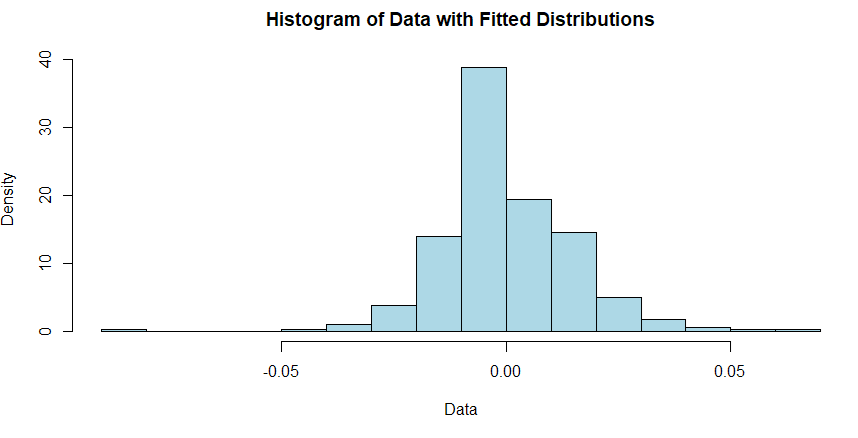
\includegraphics[width=0.8\textwidth]{./Wojtek/histogram_log_returns.png}
    \caption{Histogram logarytmicznych zwrotów}
    \label{fig:histogram_log_returns}
\end{figure}

\newpage\subsubsection{Podsumowanie:}

Przeprowadzona analiza log-zwrotów akcji spółki Wawel SA wykazała, że:

\begin{itemize}
    \item Średnia log-zwrotów jest bliska zeru, co sugeruje brak wyraźnego trendu wzrostowego lub spadkowego w badanym okresie.
    \item Odchylenie standardowe wskazuje na umiarkowaną zmienność log-zwrotów.
    \item Kwantyle pokazują asymetrię w rozkładzie log-zwrotów, co jest typowe dla danych finansowych.
    \item Rozkład normalny lepiej dopasowuje się do danych niż rozkład T-Studenta, co potwierdzają statystyki dobroci dopasowania i kryteria informacyjne.
    \item Test hipotezy metodą Monte Carlo sugeruje odrzucenie hipotezy, że dane pochodzą z rozkładu t-Studenta, wskazując na lepsze dopasowanie wyników otrzymanych z rozkładu normalnego.
\end{itemize}

\newpage\section{Analiza łącznego rozkładu log-zwrotów}

\subsection{Wstęp}
Poniższy rozdział poświęcony jest analizie wektorów log-zwrotów trzech akcji spółek: Wawel SA, Digitree oraz Vigo Photonics. Analiza zostanie przeprowadzona na parach spółek, tak aby zbadać zależności między każdą z nich.

Zakładamy, że log-zwroty akcji spółek są realizacjami zmiennych losowych, które oznaczamy jako $W, D, V$ - kolejno: Wawel, Digitree oraz Vigo Photonics. Zakładamy, żelog-zwroty dwóch akcji są niezależnymi realizacjami wektora losowego $(X,Y)$ o nieznanej gęstości $f$, wektorze średnich $(\mu_1,\mu_2)$, współczynniku korelacji $\rho$, macierzy kowariancji $\Sigma$ i macierzy korelacji $P$.

\subsection{Estymacja wektora srednich}
Z wykorzystaniem estymatora wartości oczekiwanej
$$\hat{\mu}=(\overline{X}_n, \overline{Y}_n) = (\frac{1}{n}\sum_{i=1}^{n}X_i, \frac{1}{n}\sum_{i=1}^{n}Y_i)$$
estymujemy wektor średnich log-zwrotów dla każdej pary. Otrzymujemy następujące wyniki:
$$\hat{\mu}_1=(\overline{W}_n, \overline{D}_n) = (0.0014818927, 0.0005527318)$$
$$\hat{\mu}_2=(\overline{W}_n, \overline{V}_n) = (0.001481893, -0.001203487)$$
$$\hat{\mu}_3=(\overline{V}_n, \overline{D}_n) = (-0.0012034874, 0.0005527318)$$

\subsection{Estymacja współczynnika korelacji}
Korzystając z estymatora współczynnika korelacji
$$\hat{\rho}=R_{xy}=\frac{S_{xy}}{S_x\cdot S_y}=\frac{\sum_{i=1}^{n}(X_i-\overline{X}_n)(Y_i-\overline{Y}_n)}{\sqrt{\sum_{i=1}^{n}(X_i-\overline{X}_n)^{2}}\sqrt{\sum_{i=1}^{n}(Y_i-\overline{Y}_n)^{2}}},$$
gdzie $S_x^{2}$ i $S_y^{2}$ są nieobciążonymi estymatorami wariancji
$$S^2_x=\sigma_1^2=\frac{1}{n-1}\sum_{i=1}^{n}(X_i-\overline{X}_n)^2, S^2_y=\sigma_2^2=\frac{1}{n-1}\sum_{i=1}^{n}(Y_i-\overline{Y}_n)^2$$ 
wyestymowujemy współczynnik korelacji dla każdej pary. Otrzymujemy następujące wyniki:
$$\hat{\rho}_1=R_{wd}=0.02505802$$
$$\hat{\rho}_2=R_{wv}=0.0887725$$
$$\hat{\rho}_3=R_{vd}=0.1039696$$

\subsection{Estymacja macierzy kowariancji}
Korzystając z estymatora macierzy kowariancji
$$
\hat{\Sigma}=
\begin{bmatrix}
    S^2_x & S^2_{xy} \\
    S^2_{xy} & S^2_y
\end{bmatrix}
$$
estymujemy macierz kowariancji dla każdej pary. Otrzymujemy następujące wyniki:
$$
\hat{\Sigma}_1=
\begin{bmatrix}
    S^2_w & S^2_{wd} \\
    S^2_{wd} & S^2_d
\end{bmatrix}
=
\begin{bmatrix}
    3.157575e-04 & 2.114492e-05 \\
    2.114492e-05 & 2.255094e-03
\end{bmatrix}
$$
$$
\hat{\Sigma}_2=
\begin{bmatrix}
    S^2_w & S^2_{wv} \\
    S^2_{wv} & S^2_v
\end{bmatrix}
=
\begin{bmatrix}
    0.0003157575 & 0.0000503125 \\
    0.0000503125 & 0.0010172816
\end{bmatrix}
$$
$$
\hat{\Sigma}_3=
\begin{bmatrix}
    S^2_v & S^2_{vd} \\
    S^2_{vd} & S^2_d
\end{bmatrix}
=
\begin{bmatrix}
    0.0010172816 & 0.0001574742 \\
    0.0001574742 & 0.0022550944
\end{bmatrix}
$$

\subsection{Estymacja macierzy korelacji}
Macierze korelacji
$$R=
\begin{bmatrix}
    1 & \rho \\
    \rho & 1 
\end{bmatrix}$$
dla każdej z par wyglądają następująco:
$$
R_{wd}=
\begin{bmatrix}
    1 & 0.02505802 \\
    0.02505802 & 1
\end{bmatrix}
$$
$$
R_{wv}=
\begin{bmatrix}
    1 & 0.0887725 \\
    0.0887725 & 1
\end{bmatrix}
$$
$$
R_{vd}=
\begin{bmatrix}
    1 & 0.1039696 \\
    0.1039696 & 1
\end{bmatrix}
$$

\newpage\subsection{Wykresy rozrzutów z histogramami rozkładów brzegowych}
Poniżej przedstawione zostały wykresy rozrzutów z histogramami rozkładów brzegowych dla każdej z par spółek:

\begin{figure}[!htb]
\minipage{0.5\textwidth}
  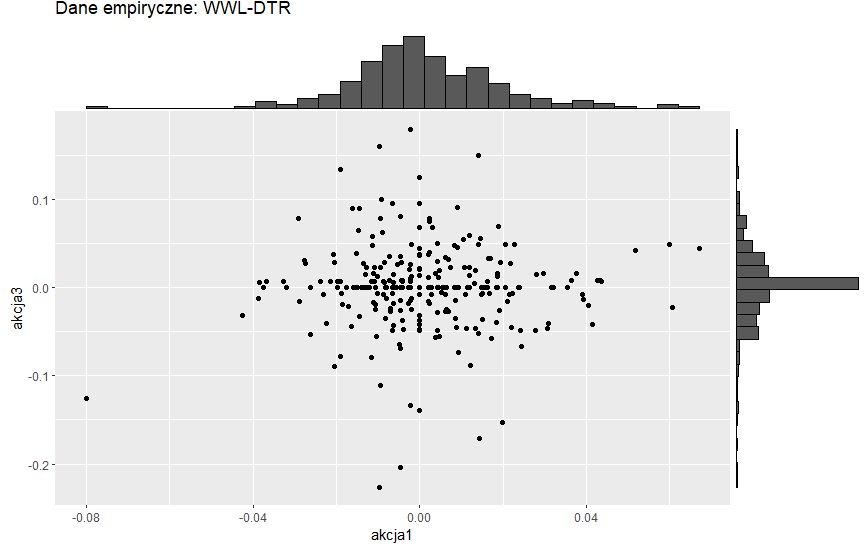
\includegraphics[width=\linewidth]{./img/dane empiryczne-wwl-dtr.png}
\endminipage\hfill
\minipage{0.5\textwidth}
  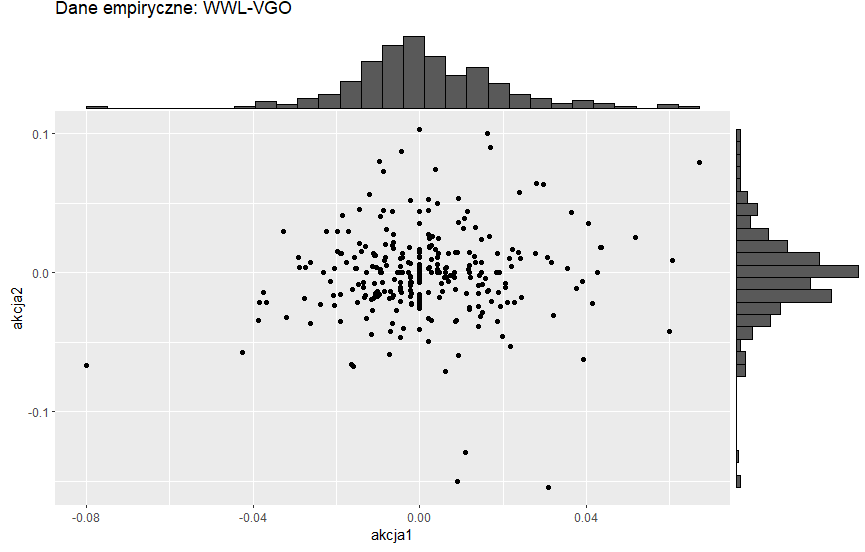
\includegraphics[width=\linewidth]{./img/dane empiryczne-wwl-vgo.png}
\endminipage\hfill
\end{figure}
\begin{figure}[H]
    \centering
    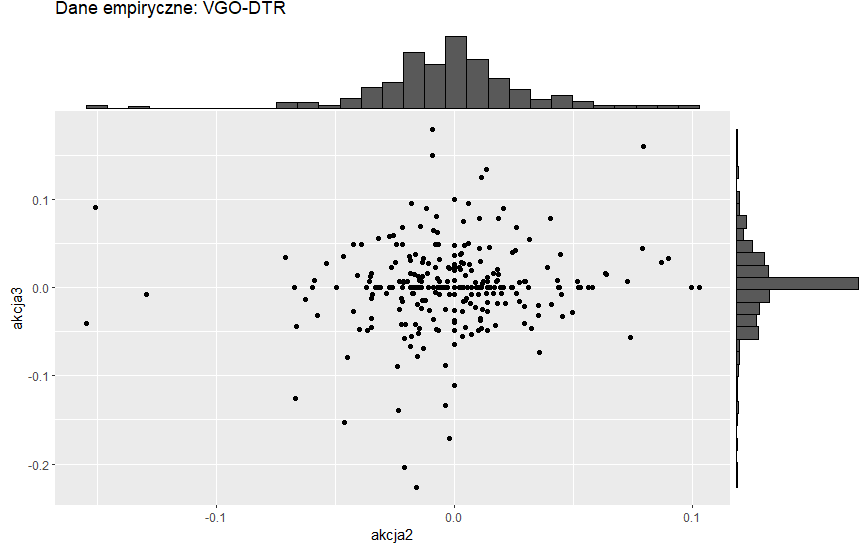
\includegraphics[width=0.5\textwidth]{./img/dane empiryczne-vgo-dtr.png}
\end{figure}

Punkty koncentrują się w okolicach wartości zerowych, sugerując niewielkie wahania dzienne. Rozkłady pozostają stabilne, a obserwacje nie wskazują na znaczące zniekształcenia lub nieliniowości.

\subsection{Wzór gęstości rozkładu normalnego}
Wzór gęstości rozkładu normalnego o wyestymowanych wcześniej parametrach:
$$f(x_1,x_2)=\frac{1}{2\pi\sigma_1\sigma_2\sqrt{1-\rho^2}}\exp\left(-\frac{1}{2(1-\rho^2)}\left[\frac{(x_1-\mu_1)^2}{\sigma_1^2}-2\rho\frac{(x_1-\mu_1)(x_2-\mu_2)}{\sigma_1\sigma_2}+\frac{(x_2-\mu_2)^2}{\sigma_2^2}\right]\right)$$
dla każdej z par wygląda następująco:

$$f(w,d)=\frac{1}{0.005300327}
\exp\left(-\frac{1}{1.999372} 
\left[\frac{(x_1-0.0014818927)^2}{3.157575e-04}-0.05011604\frac{(x_1-0.0014818927)(x_2-0.0005527318)}{0.0008438382}+\frac{(x_2-0.0005527318)^2}{2.255094e-03}\right]\right)$$

$$f(w,v)=\frac{1}{2\pi\sigma_1\sigma_2\sqrt{1-\rho^2}}\exp\left(-\frac{1}{2(1-\rho^2)}\left[\frac{(x_1-\mu_1)^2}{3.157575e-04}-2\rho\frac{(x_1-\mu_1)(x_2-\mu_2)}{\sigma_1\sigma_2}+\frac{(x_2-\mu_2)^2}{\sigma_2^2}\right]\right)$$
$$f(v,d)=\frac{1}{2\pi\sigma_1\sigma_2\sqrt{1-\rho^2}}\exp\left(-\frac{1}{2(1-\rho^2)}\left[\frac{(x_1-\mu_1)^2}{\sigma_1^2}-2\rho\frac{(x_1-\mu_1)(x_2-\mu_2)}{\sigma_1\sigma_2}+\frac{(x_2-\mu_2)^2}{\sigma_2^2}\right]\right)$$
\newpage Wykresy gęstości łącznej prezentują się następująco:

\begin{figure}[!htb]
\minipage{0.5\textwidth}
  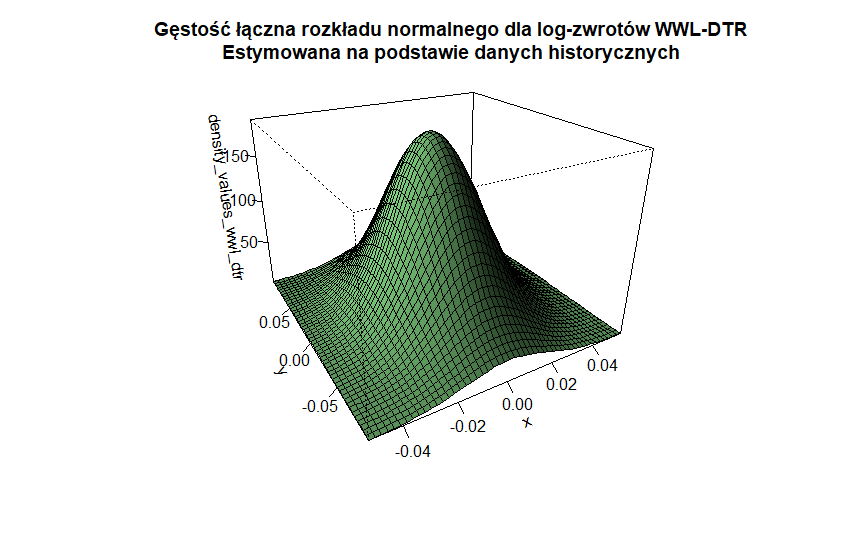
\includegraphics[width=\linewidth]{./img/gestosc-laczna-wwl-dtr.png}
\endminipage\hfill
\minipage{0.5\textwidth}
  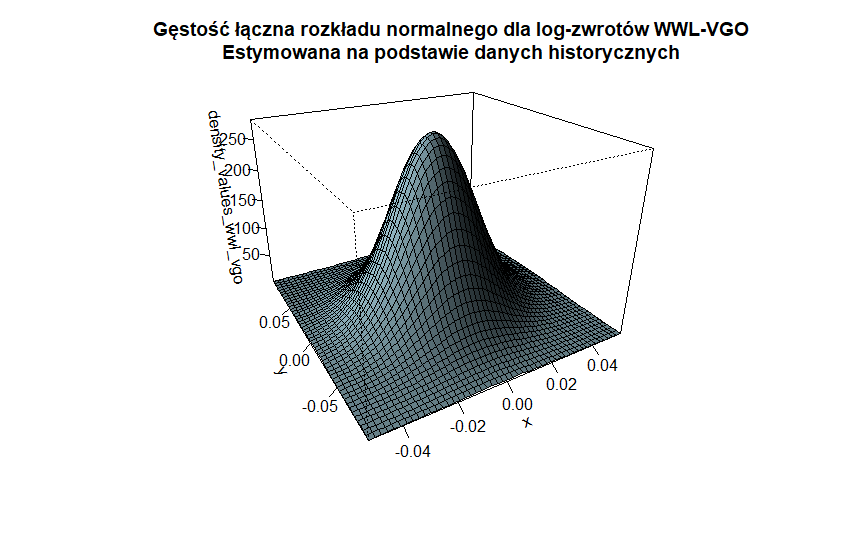
\includegraphics[width=\linewidth]{./img/gestosc-laczna-wwl-vgo.png}
\endminipage\hfill
\end{figure}
\begin{figure}[H]
    \centering
    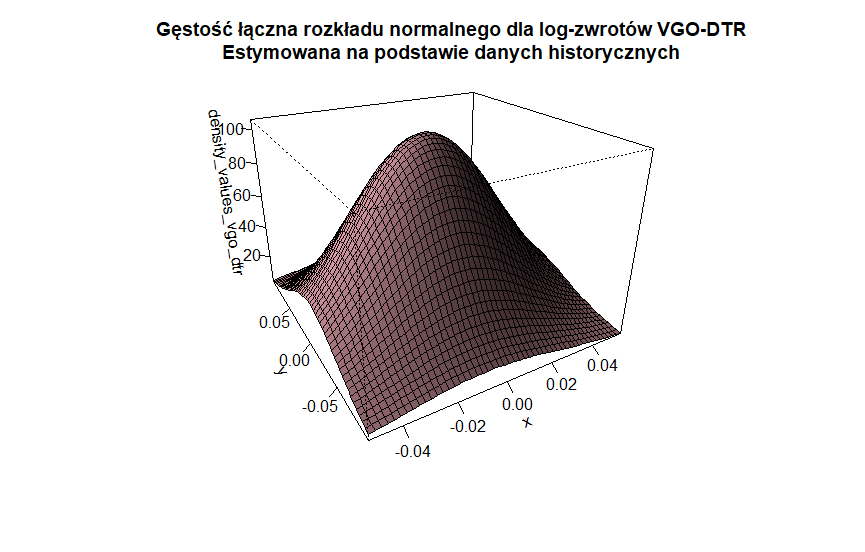
\includegraphics[width=0.5\textwidth]{./img/gestosc-laczna-vgo-dtr.png}
\end{figure}

Każdy wykres to trójwymiarowa powierzchnia, gdzie na osi poziomej oraz głębokościowej (x i y) umieszczono wartości logarytmicznych zmian cen poszczególnych spółek, a na osi pionowej (z) zaprezentowano wartość gęstości prawdopodobieństwa wynikającą z przyjętego modelu rozkładu normalnego dwuwymiarowego. Kształt powierzchni z wyraźnym szczytem sugeruje, że najbardziej prawdopodobne wartości to niewielkie dzienne zmiany cen obu analizowanych aktywów. W miarę oddalania się od punktu (0,0) w stronę większych lub mniejszych stóp zwrotu, wysokość powierzchni opada, wskazując na mniejsze prawdopodobieństwo wystąpienia takich skrajnych zdarzeń. 

\subsection{Wzory gęstości rozkładów brzegowych}
Korzystając z zależności
$$f_1(x)=\int_{-\infty}^{\infty}f(x,y)dy, f_2(y)=\int_{-\infty}^{\infty}f(x,y)dx,$$
wyznaczamy wzory gęstości rozkładów brzegowych dla każdej pary.\\ Otrzymujemy:
$$f_1(x)=$$
$$f_2(x)=$$
$$f_3(x)=$$
Poniżej przedstawiono wykresy gęstości rozkładów brzegowych:
\begin{figure}[H]
    \centering
    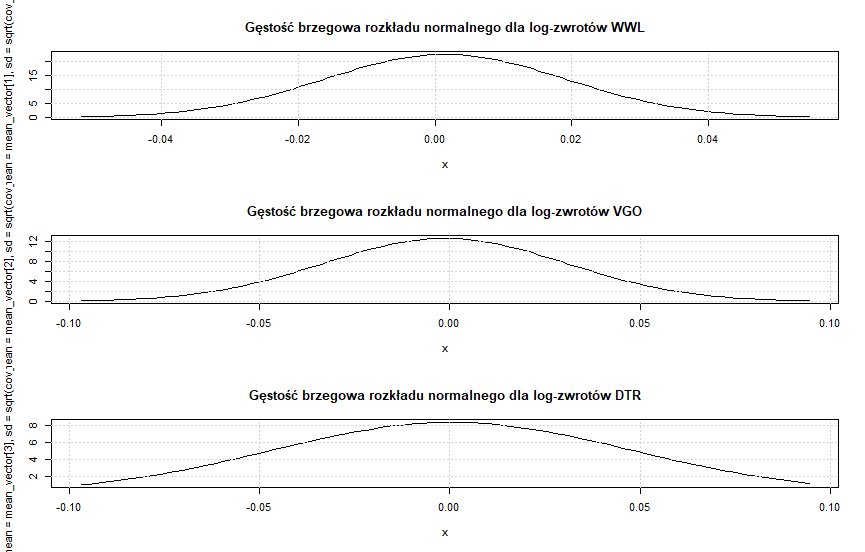
\includegraphics[width=1\textwidth]{./img/gestosci-brzegowe.png}
\end{figure}
Rozkłady marginalne poszczególnych spółek są dobrze aproksymowane przez rozkład normalny – krzywe mają kształt zbliżony do krzywej Gaussa. Szczyt gęstości w okolicach zera ponownie potwierdza niewielkie, dominujące dzienne zmiany cen.

\subsection{Wstępna ocena dobroci rozkładu normalnego z wyestymowanymi parametrami}
Wygenerowano próbę liczności danych z rozkładu normalnego z wyestymowanymi wcześniej parametrami. W tej części porównane zostaną wykresy rozrzutu wygenerowanych prób z wykresami rozrzutu danych i na ich podstawie oceniona zostanie wstępnie dobroć rozkładu normalnego dla wyestymowanych parametrów.

\begin{figure}[H]
    \centering
    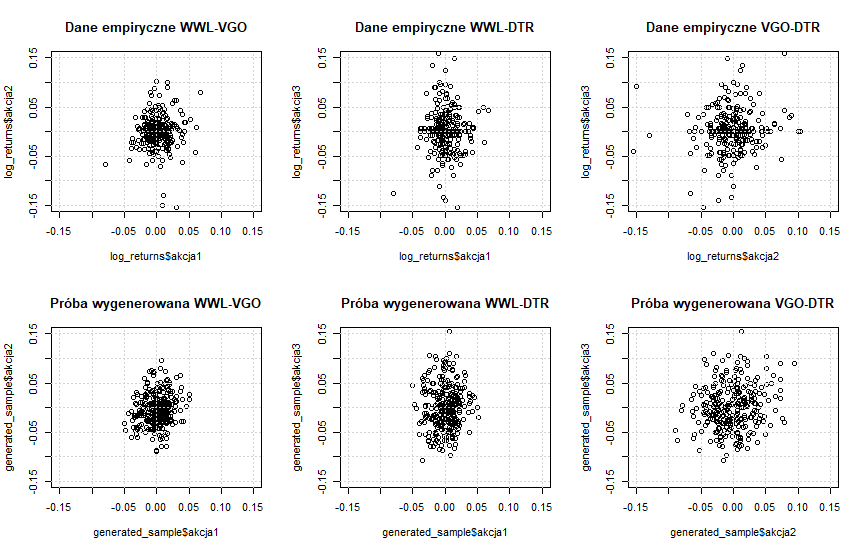
\includegraphics[width=1\textwidth]{./img/dane empiryczne-proba wygenerowana pary.png}
\end{figure}

W przypadku pary WWL-VGO Dane empiryczne i dane wygenerowane wykazują podobną strukturę rozrzutu logarytmicznych stóp zwrotu, co sugeruje, że rozkład normalny z parametrami wyestymowanymi wcześniej jest dobrze dopasowany do prawdziwych danych. W przypadku par WWL-DTR oraz VGO-DTR, można zauważyć rozbieżności w skrajnych przypadkach.

\end{document}